\Chapter{Közbülső reprezentáció}

A keresztfordító működése szerint beolvassa a nyelvi fájlt, melyet a programozó a definiált nyelven megírt, majd szekvenciálisan feldolgozza azt. A szinkatkikai elemzés után egy belső szerkezet jön létre, mely leírja a beolvasott programkódot.

A kód a belső szerkezetben osztályokba lesz szervezve, ezekről az alábbiakban kerül említésre néhány információ.

\begin{figure}
\centering
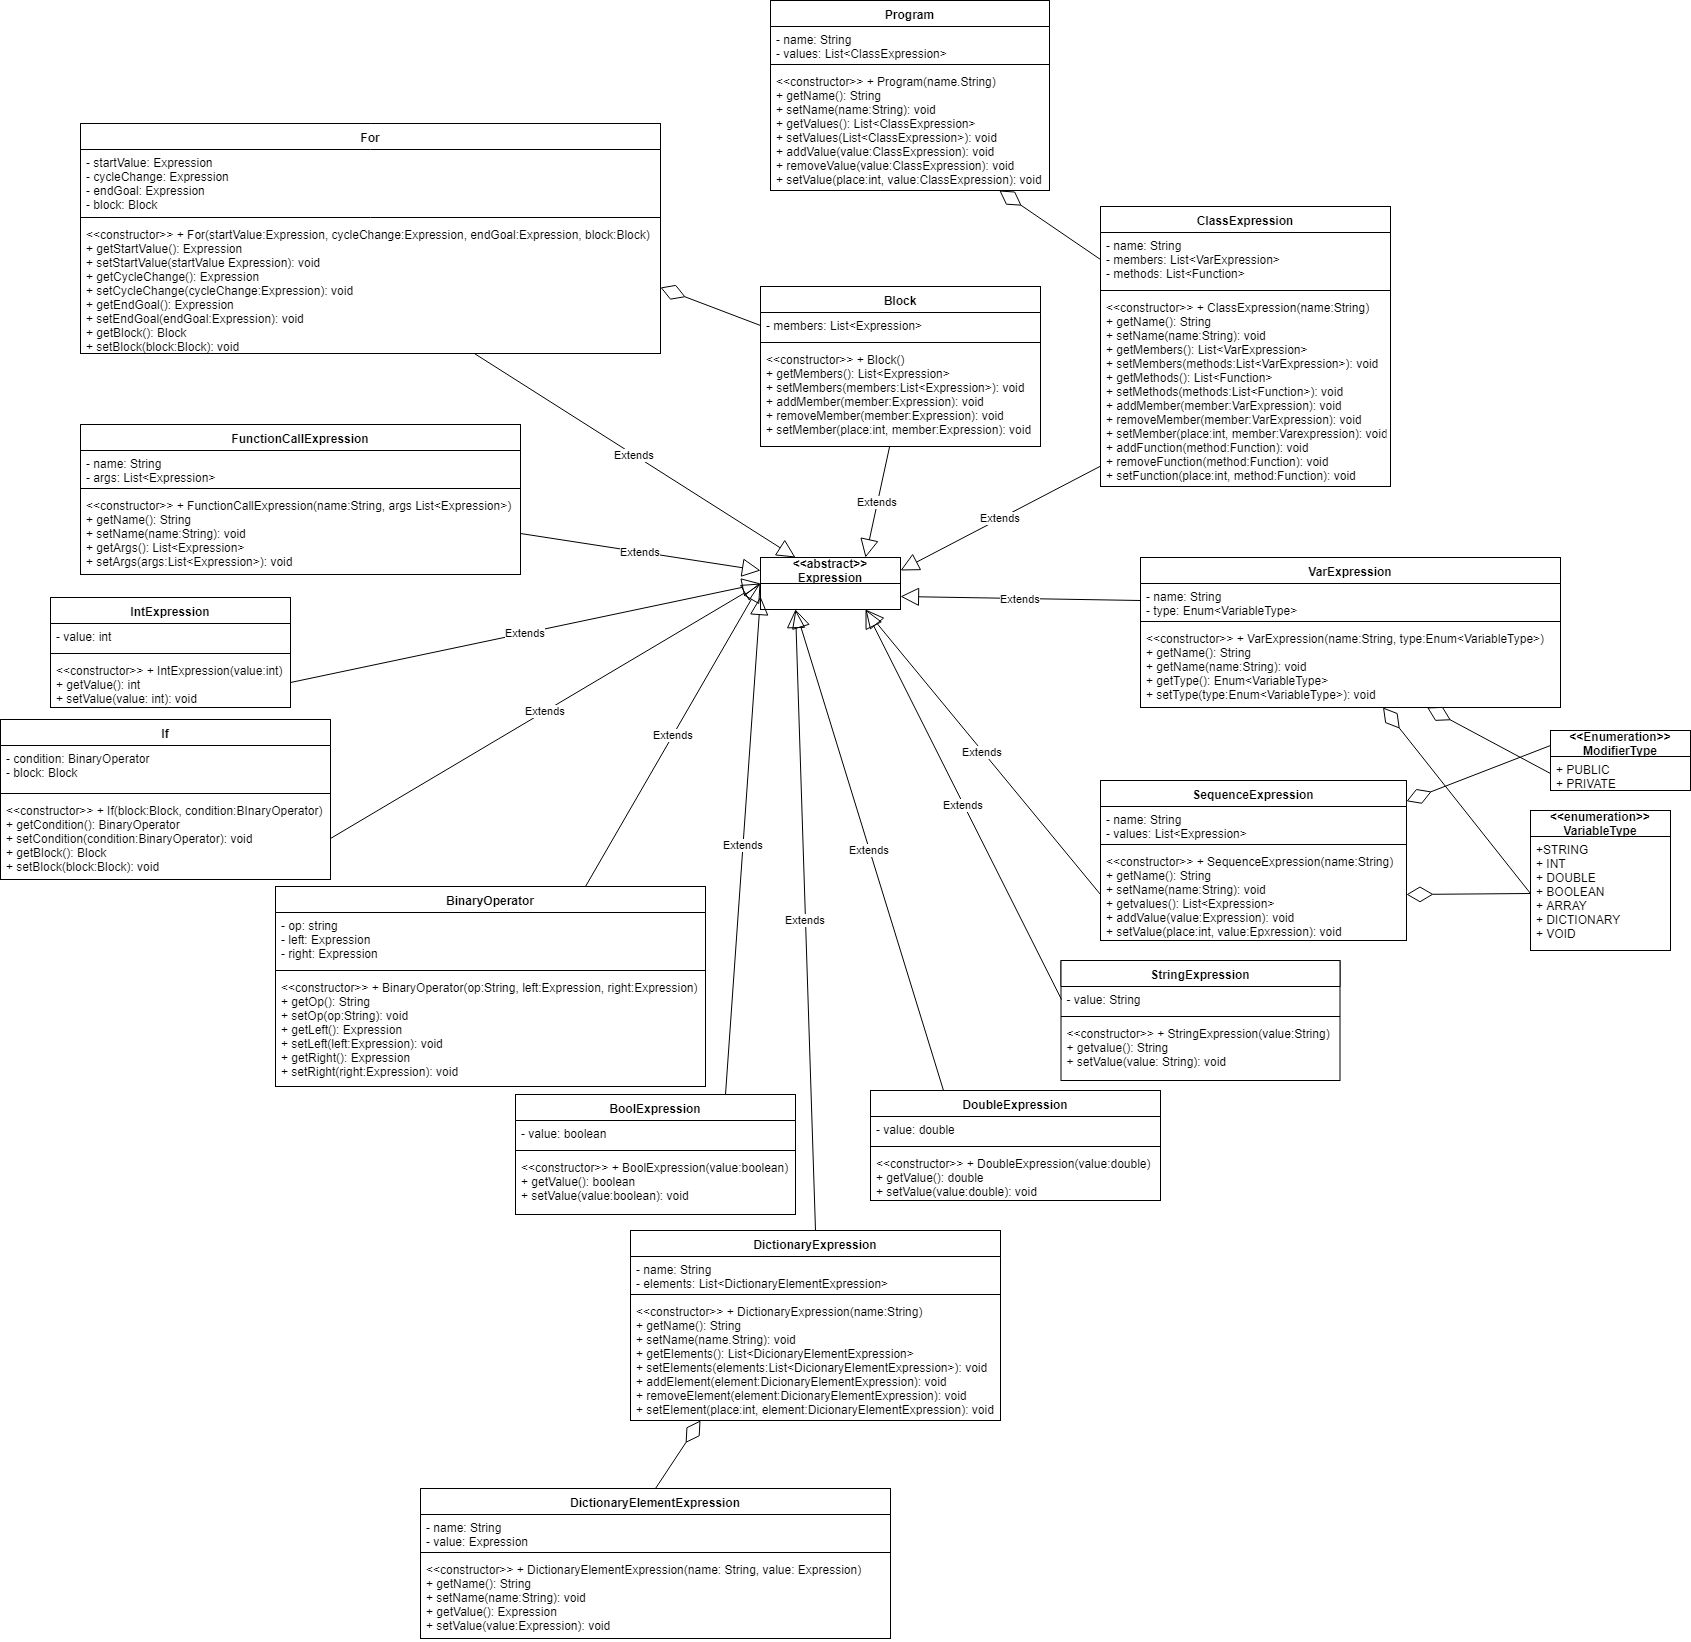
\includegraphics[scale=1]{kepek/rr_uml.png}
\caption{Osztálydiagram}
\label{fig:process}
\end{figure}

\begin{itemize}
\item függvénydefiníció
\begin{figure}
\centering
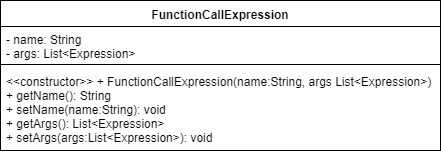
\includegraphics[scale=1]{kepek/rr_funccallexpr_dia.png}
\caption{Függvényhívás}
\label{fig:process}
\end{figure}
\item változó definíció
\begin{figure}
\centering
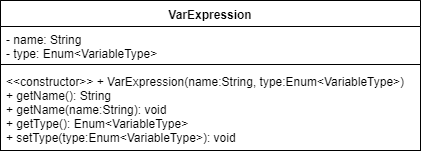
\includegraphics[scale=1]{kepek/rr_var_dia.png}
\caption{Változó osztály}
\label{fig:process}
\end{figure}
\item for ciklus
\begin{figure}
\centering
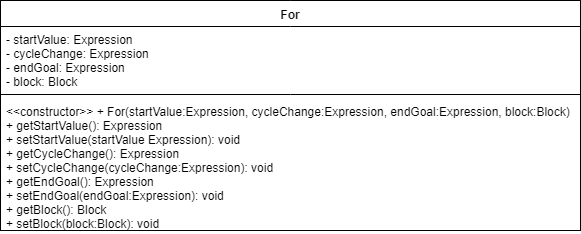
\includegraphics[scale=1]{kepek/rr_for_dia.png}
\caption{For ciklus osztálya}
\label{fig:process}
\end{figure}
\item feltételes elágazás
\begin{figure}
\centering
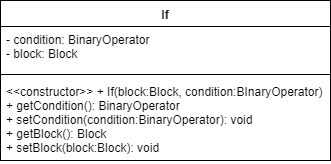
\includegraphics[scale=1]{kepek/rr_if_dia.png}
\caption{Feltételes elágazás, If osztálya}
\label{fig:process}
\end{figure}
\item osztály definíció
\begin{figure}
\centering
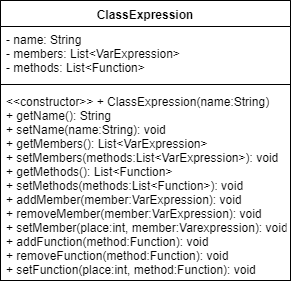
\includegraphics[scale=1]{kepek/rr_class_dia.png}
\caption{Osztály leírása osztályban}
\label{fig:process}
\end{figure}
\item program/modul/package definíció (befoglaló típusnak)
\begin{figure}
\centering
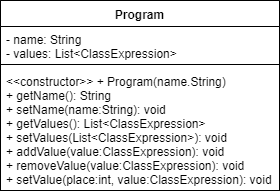
\includegraphics[scale=1]{kepek/rr_prog_dia.png}
\caption{Program osztály}
\label{fig:process}
\end{figure}
\item blokk/szekvencia típus
\begin{figure}
\centering
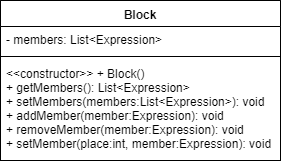
\includegraphics[scale=1]{kepek/rr_block_dia.png}
\caption{A keresztfordítás lépései}
\label{fig:process}
\end{figure}
\item expression/statement

\end{itemize}

% TODO: Jó sok UML diagram

% TODO: Absztrakt gyár mintát érdemes lesz majd bemutatni a kimeneti programnyelvek implementációjánál.
